\section{eo\-Random\-Select$<$ EOT $>$ Class Template Reference}
\label{classeo_random_select}\index{eoRandomSelect@{eoRandomSelect}}
eo\-Random\-Select: a selection method that selects ONE individual randomly  


{\tt \#include $<$eo\-Random\-Select.h$>$}

Inheritance diagram for eo\-Random\-Select$<$ EOT $>$::\begin{figure}[H]
\begin{center}
\leavevmode
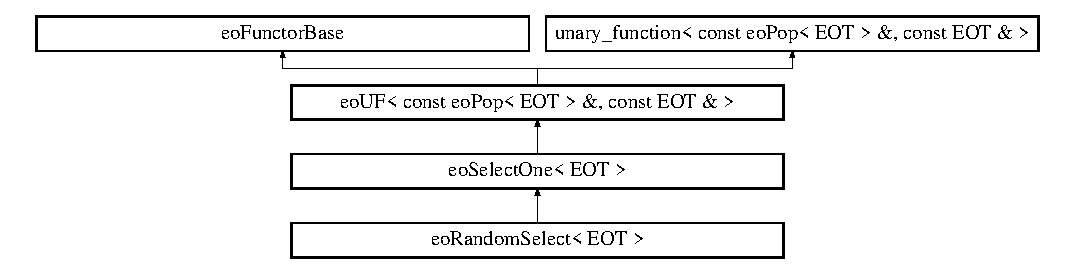
\includegraphics[height=3.23699cm]{classeo_random_select}
\end{center}
\end{figure}
\subsection*{Public Member Functions}
\begin{CompactItemize}
\item 
virtual const {\bf EOT} \& {\bf operator()} (const {\bf eo\-Pop}$<$ {\bf EOT} $>$ \&\_\-pop)\label{classeo_random_select_a0}

\begin{CompactList}\small\item\em not a big deal!!! \item\end{CompactList}\end{CompactItemize}


\subsection{Detailed Description}
\subsubsection*{template$<$class EOT$>$ class eo\-Random\-Select$<$ EOT $>$}

eo\-Random\-Select: a selection method that selects ONE individual randomly 



Definition at line 44 of file eo\-Random\-Select.h.

The documentation for this class was generated from the following file:\begin{CompactItemize}
\item 
eo\-Random\-Select.h\end{CompactItemize}
